\documentclass[10pt,a4paper]{article}
\usepackage[utf8]{inputenc}
\usepackage[francais]{babel}
\usepackage[T1]{fontenc}
\usepackage{amsmath}
\usepackage{amsfonts}
\usepackage{amssymb}
\usepackage{makeidx}
\usepackage{graphicx}
\usepackage{float} %pour que l'option "H" fonctionne dans figure.
\usepackage[left=2cm,right=2cm,top=2cm,bottom=2cm]{geometry}
\usepackage{hyperref} % lien hypertext
%\hypersetup{pdfborder={0 0 0}}

\begin{document}
%\setcounter{page}{1} % enlever numero de page


\begin{minipage}{0.5\linewidth} % permet de faire les deux colonnes pour mettre l'image à  droite du texte
Colpier Clément\\
Fornarat Thibault\\
Pellegrino Guillaume\\
Renard Charles\\



26/01/13
\end{minipage}
\begin{minipage}{0.5\linewidth}
\begin{flushright}

\includegraphics[scale=0.2]{logo-esiee.jpg}

\end{flushright}
\end{minipage}


\vspace{8cm}

\begin{center}
\LARGE Projet de Mathématiques appliquées \\
\-
\LARGE PR3003
\\

\end{center}




\newpage
-
\newpage
\tableofcontents              % Table des matieres
\clearpage


\section{Déterminer l'équation différentielle vérifiée par M(t)=(x(t),y(t)).}
\begin{figure}[H]
	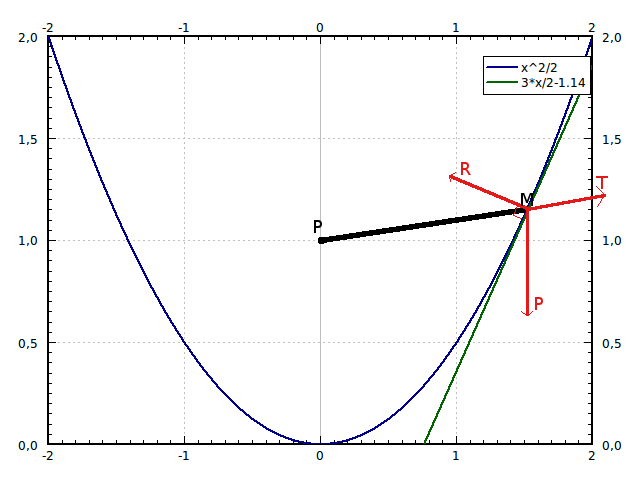
\includegraphics[scale=0.7]{GraphMath2.png}
	%\caption{Histoire de Sanofi}
\end{figure}
La masselotte M se déplace uniquement selon la composante tangentielle. Pour déterminer l'équation différentielle on va donc particulièrement s'intéresser à l'équation sur la composante tangentielle.\\
Pour cela, on commence à faire la somme des forces s'exerçant sur la composante tangentielle $\vec{u_t}$ et normale $\vec{u_n}$:
\[
   \left \{
   \begin{array}{r c l}
      mg_t+T_t=ma_t  \\
      mg_n+R_n+T_n=0 
   \end{array}
   \right .
\]
On s'intéresse à l'équation: $mg_t+T_t=ma_t$ \\ 
Pour déterminer l'équation différentielle, on doit alors projeter $\vec{T}$ et  $\vec{mg}$ sur $\vec{u_t}$. \\
On projette $\vec{mg}=-mg.\vec{u_y}$ sur $\vec{u_t}$\\

\subsubsection{Projection du Poids sur la composante tangentielle}
\begin{figure}[H]
	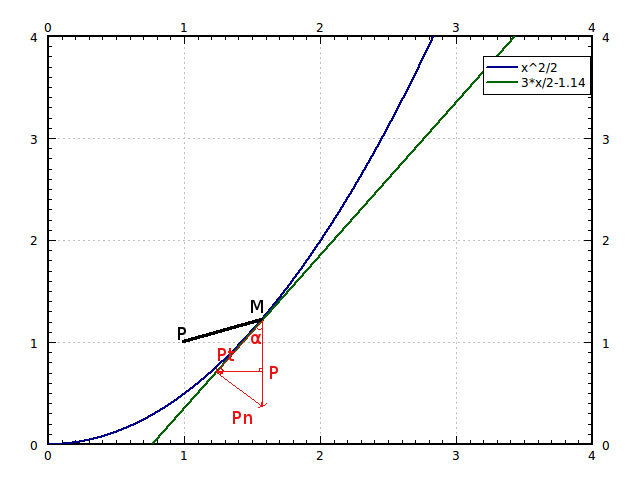
\includegraphics[scale=0.7]{GraphMathZoomProjectionPoids.png}
	%\caption{Histoire de Sanofi}
\end{figure}

On remarque sur le graphique que $P_t=P.\cos(\alpha)$\\
On cherche à déterminer $\alpha$.
On calcule la pente a de la tige parabolique. $a=\frac{\partial y}{\partial x}=\frac{\partial x^2/2}{\partial x}=x$ \\
En $M(x_0,y_0)$ la pente a de la tige parabolique vaut donc $x_0$.
Cette pente a nous permet de calculer l'angle $\alpha$. En effet, on remarque graphiquement que $\tan(\alpha)=\frac{a}{1}$. On en déduit: $\alpha=\tan^{-1}(x_0)$\\
Au final on trouve donc: $P_t=P.\cos(\tan^{-1}(x_0)) $\\
$\cos(\tan^{-1}(x))=\frac{1}{1+x^2}$ ( A vérifier) Donc: $P_t=P.\frac{1}{1+x^2_0}$
\\
On projette désormais $\vec{T}$ sur $\vec{u_t}$. Il faut pour cela d'abord projeter $\vec{T}$ sur $\vec{u_x}$ et $\vec{u_y}$. \\

\subsubsection{Projection de la tension du ressort su la composante tangentielle}
\begin{figure}[H]
	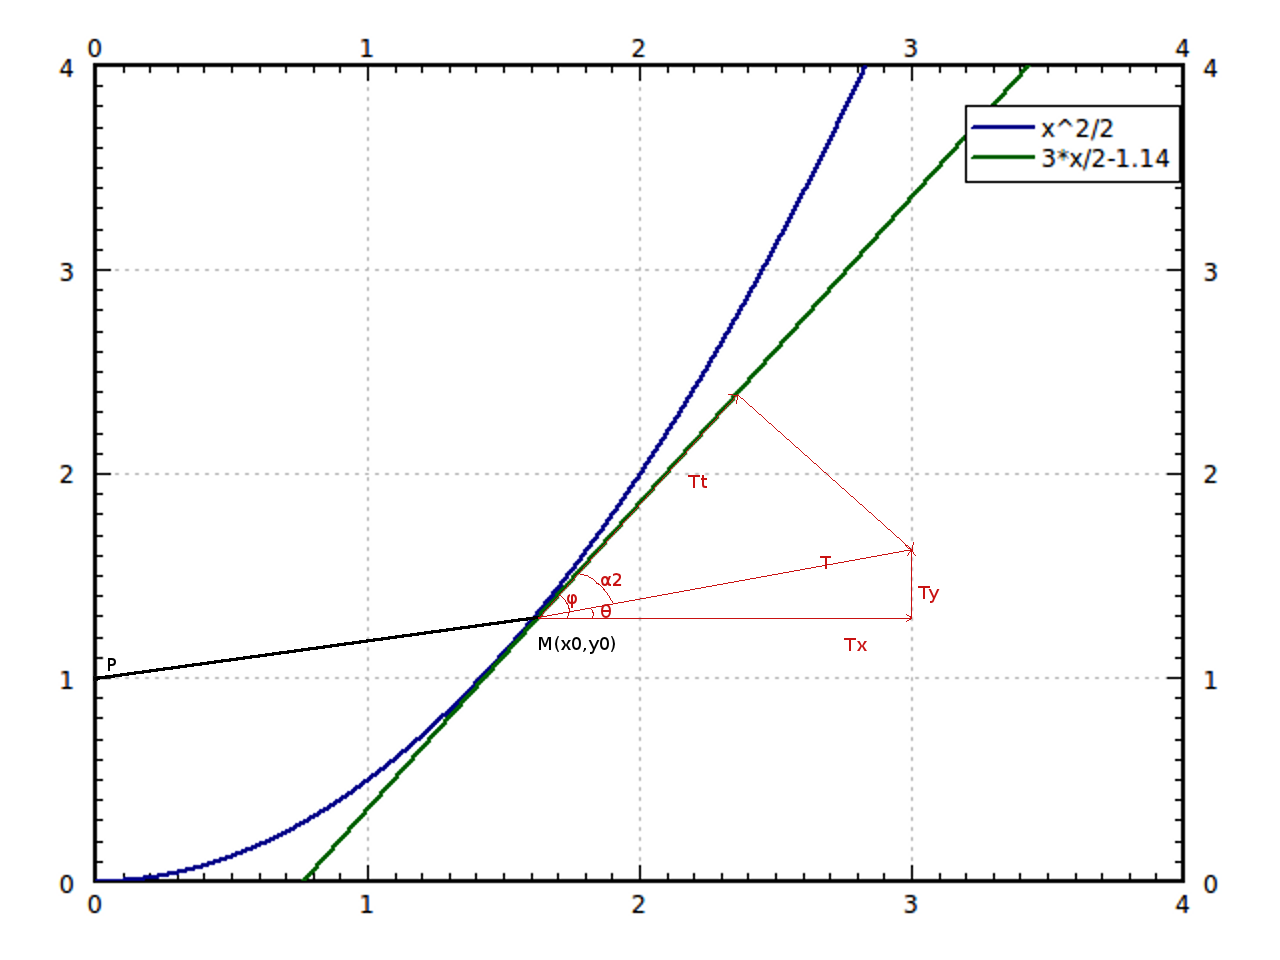
\includegraphics[scale=0.35]{GraphMathZoomProjectionT.png}
	%\caption{Histoire de Sanofi}
\end{figure} 

La pente de la tangente vaut $x_0$. Celle de $\vec{PM}$ vaut $\frac{y_0-1}{x_0}$.\\
On en déduit ainsi: $\tan(\phi)=x_0$ et $\tan(\theta)=\frac{y_0-1}{x_0}$
On obtient ainsi $\alpha=\tan^{-1}(x_0) - \tan^{-1}(\frac{y_0-1}{x_0})$ et on en déduit: $T_t=T.\cos(\tan^{-1}(x_0) - \tan^{-1}(\frac{y_0-1}{x_0}))$



\end{document}